\documentclass[12px]{article}
\usepackage{graphicx} % Required for inserting images

\usepackage[T2A]{fontenc}
\usepackage[utf8]{inputenc}
\usepackage[english, russian]{babel}
\usepackage{amsmath}

\usepackage{geometry}
 \geometry{
 a4paper,
 total={170mm,257mm},
 left=20mm,
 top=20mm,
 }

\title{ЭВМ}
\author{VG6}

\begin{document}

\maketitle

\section{До этого мне было лень}
\section*{Вопросики (23 октября 2025)}
Какой принцип Неймана позволяет привесить скорость света?\\
Вычислительный процесс следует организовывать параллельным образом.\\
Почему ЭВМ в двоичной системе счисления, а не в десятичной?\\
5 принцип Неймана: разработка устройств для других операция нецелесообразно (кроме сумматора). В теории он прав, а на практике нет. К примеру аппаратные умножители. \\
\textbf{Главный принцип Неймана}: и программа и данные лежат в одном и том же месте в одном и том же виде. Не нужно для заменять машину, можно заменить только программу. \\
\textbf{Схема} - графическое обозначение элементов и связи между ними. \\

\section{Структура классической ЭВМ.}
Состоит из 3х блоков.
\begin{center}
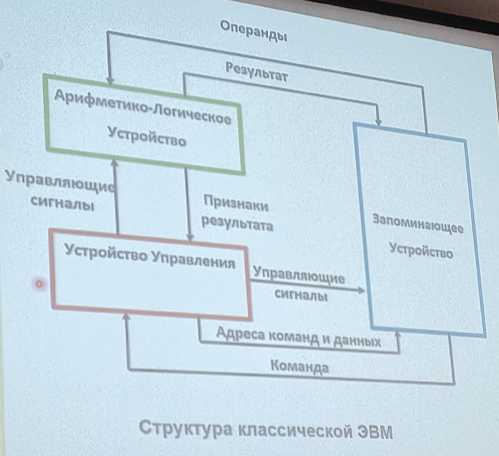
\includegraphics[width=0.7\linewidth]{images/Схема ЭВМ.png}
\end{center}

\subsection{Описание блоков.}
\begin{enumerate}
    \item Арифметико-Логическое устройство
    \begin{itemize}
        \item Выполняет преобразование информации представленной в двоичном виде. Например: числа при выполнении арифметической операции. 
        \item \textbf{Операнд} - мы будем называть участника арифметической или логической операции. 
        \item АЛУ преобразует операнды и получает результат и признаки результат (дополнительные сведенья о том, какй результат получился Правильный/Неправильный).
        \item Какой операцией заняться определяют управляющие сигналы.
        \item \textbf{Операция} - арифметическое или логическое действие выполняемое в АЛУ над операндами. То, что может делать АЛУ называется операцией.
    \end{itemize}
    \item Запоминающее устройство
    \begin{itemize}
        \item Предназначение: хранить двоичные числа.\\
        Для этого нужны 3 операции:
        \begin{enumerate}
            \item Запись
            \item Чтение
            \item Выборка (адресация не совсем одно и тоже)
        \end{enumerate}
        \item Запоминающее устройство классической ЭВМ является адресным устройством. Каждое число хранится в ячейке имеющей свой уникальный адрес, который тоже является числом. В простейшем случае - порядковый номер ячейки памяти.
        \item Запоминающее устройство представляет собой одномерный массив, где в качестве индекса выступает адрес (номер ячейки).
        \item 4 действия (тоже + хранение) определяется управляющими сигналами, среди которых сигналы: операции записи, чтения и многое другое. 
    \end{itemize}
    \item Устройство Управления
    \begin{itemize}
        \item Занимается управлением вычислительным процессом. Тоесть его выходом является порождение управляющих сигнаов (сигналов управления), которые потребляются другими ящиками и самим собой. 
        \item Помимо внешних блоков он управляет и самим собой.
        \item Цели и задачи управления: реализация выполнения команды. Для этого формируемые им сигналы несут 2 сущности: что делать, когда это надо сделать.
        \item Эту команду откуда-то надо взять. А они лежат в запоминающем устройстве, там же, где и данные. 
        \item На выходе сигналы, на входе ... из памяти
        \item нужно формировать адресс ячейки откуда взять команду, получить её и выполнить.
    \end{itemize}
\end{enumerate}
Связи между этими блоками изображены на рисунке.
По признакам результата УУ влияет на дальнейшее прохождение вычислительного процесса (изменять последовательность выполнения команд).\\\\
Например, произошло переполнение, значит нужно сформировать признак переполнения и передать УУ.\\\\
УУ получает команды из памяти, однако и операнды и команды лежат в разных ячейках запоминающего устройства (адресам) поэтому УУ должен формировать адреса как команд, так и операнд.
\subsection{Цикл выполнения команды.}
Структура организована циклически. И этот бег по кругу является бесконечным повторением. \\

\subsection{Память. Запоминающее устройство.}
Строится по иерархическому приципу.
\textbf{Регистр} - запоминающее устройство ёмкостью в 1 число. Есть 2 типа:
\begin{enumerate}
    \item Специальзированные регистры, функции которых предопределены конструкцией ЭВМ и являются неизменными и регистры 
    \item Общего назначения, функционал которых может предопределятся. Доступны для программистов.
\end{enumerate}
\subsubsection{Виды памяти}
\textbf{Сверхоперативные ЗУ} - обычно безадресного типа. К таким устройствам относятся буферные запоминающие устройства, стек.\\
\textbf{Буфер} - запоминающее устройство между ЗУ с разной скоростью работы для сглаживаний по времени. Обычно организуется очередью (FIFO).\\
\textbf{Стек} - первым вылетает последний заряженный патрон. (LIFO). История перехода к подпрограммам. Используется в системе прерываний.\\
\textbf{Постоянное запоминающее устройство (ROM)} - адресное запоминающее устройство без функции записи.
\textbf{EPROM} - оставляет возможность сменить содержимое путём перезаписи, что требует специальное устройство (программатор).\\
\textbf{КЭШ L1, L2, L3, L4} - безадрессное ассоциативное запоминающее устройство. Небольшая ёмкость, но кратно ускоряет скорость работы вычислительного устройства. Благодаря ассоциативному доступу (тэгами) аккумулируют в себе те команды или данные, которые используются наиболее интенсивно. Тем самым создавая копию ячеек Оперативной памяти кратно уменьшают доступ к этим данным.\\
\textbf{\textit{Основная оперативна память ООП}, ОЗУ, RAM, память с произвольной выборкой, память ЭВМ} - (синенькое на схеме) память, в которой хранятся те самые команды и данные по Нейману.\\
\textbf{Специализированные блоки памяти} - обмен между вычислительным ядром внешним миром (многопортовая память, ассоциативные ЗУ (используется в КЭШе и т.д. при поиске не по адресу, а по признаку), видеопамять)\\
\textbf{Внешние запоминающие устройства} - то, что подключается к ... через интерфейс. (..., облачные зранилища, Data-центры, ...)

\subsection{ОЗУ. Оперативное запоминающее устройтсво.}
Совокупность ячеек, пре
данный вид памяти для работы в качестве основной опреративной памяти ЭВМ дляжно обладать свойством произвольной выборки. \\

\textbf{Памятью с произвольной выборкой} мы будем называть адресное ЗУ, время выборки которого не зависит от адреса ячейки и последовательности обращений к ячейкам этого устройства.\\

Технические характеристики ЗУ: 
\begin{itemize}
    \item 1 бит - 1 двоичный разряд
    \item 1 байт - 8 бит. Попытка представить символы алфавита при помощи таблички кодирования (ASCII).
    \item К(Кило) - $2^{10} = 1024$
    \item М(Мега) - $2^{20} = ... $ 
    \item Г(Гига) - $2^{30} = ... $
\end{itemize}

\textbf{Память} - информационная ёмкость 1 адресуемой ячейки того, что имеет адрес. \\

\textbf{Организация ЗУ} - произведение числа ячеек на их разрядность, например: 4Гx8\\
Характеристики запоминающего устройства - временные.\\

\textbf{Быстродействие (производительность) ЗУ} - оценивают временами считывания и записи, длительностью циклов считывания/записи

\textbf{Время считывания} — интервал времени между моментом сигнала на считывание (адрес или разрешение считывания) и моментом выдачи данных на выходы памяти.

\textbf{Время записи} - интервал времени после задания сигнала записи, достаточный для установления ячейки в состояние, задаваемое входными данными.

\textbf{Цикл считывания/записи} - минимальный интервал между последовательными обращениями.
\subsection{Примеры условных графических обозначений (УГО ЗУ)}
Запоминающее устройство:
\begin{center}	
	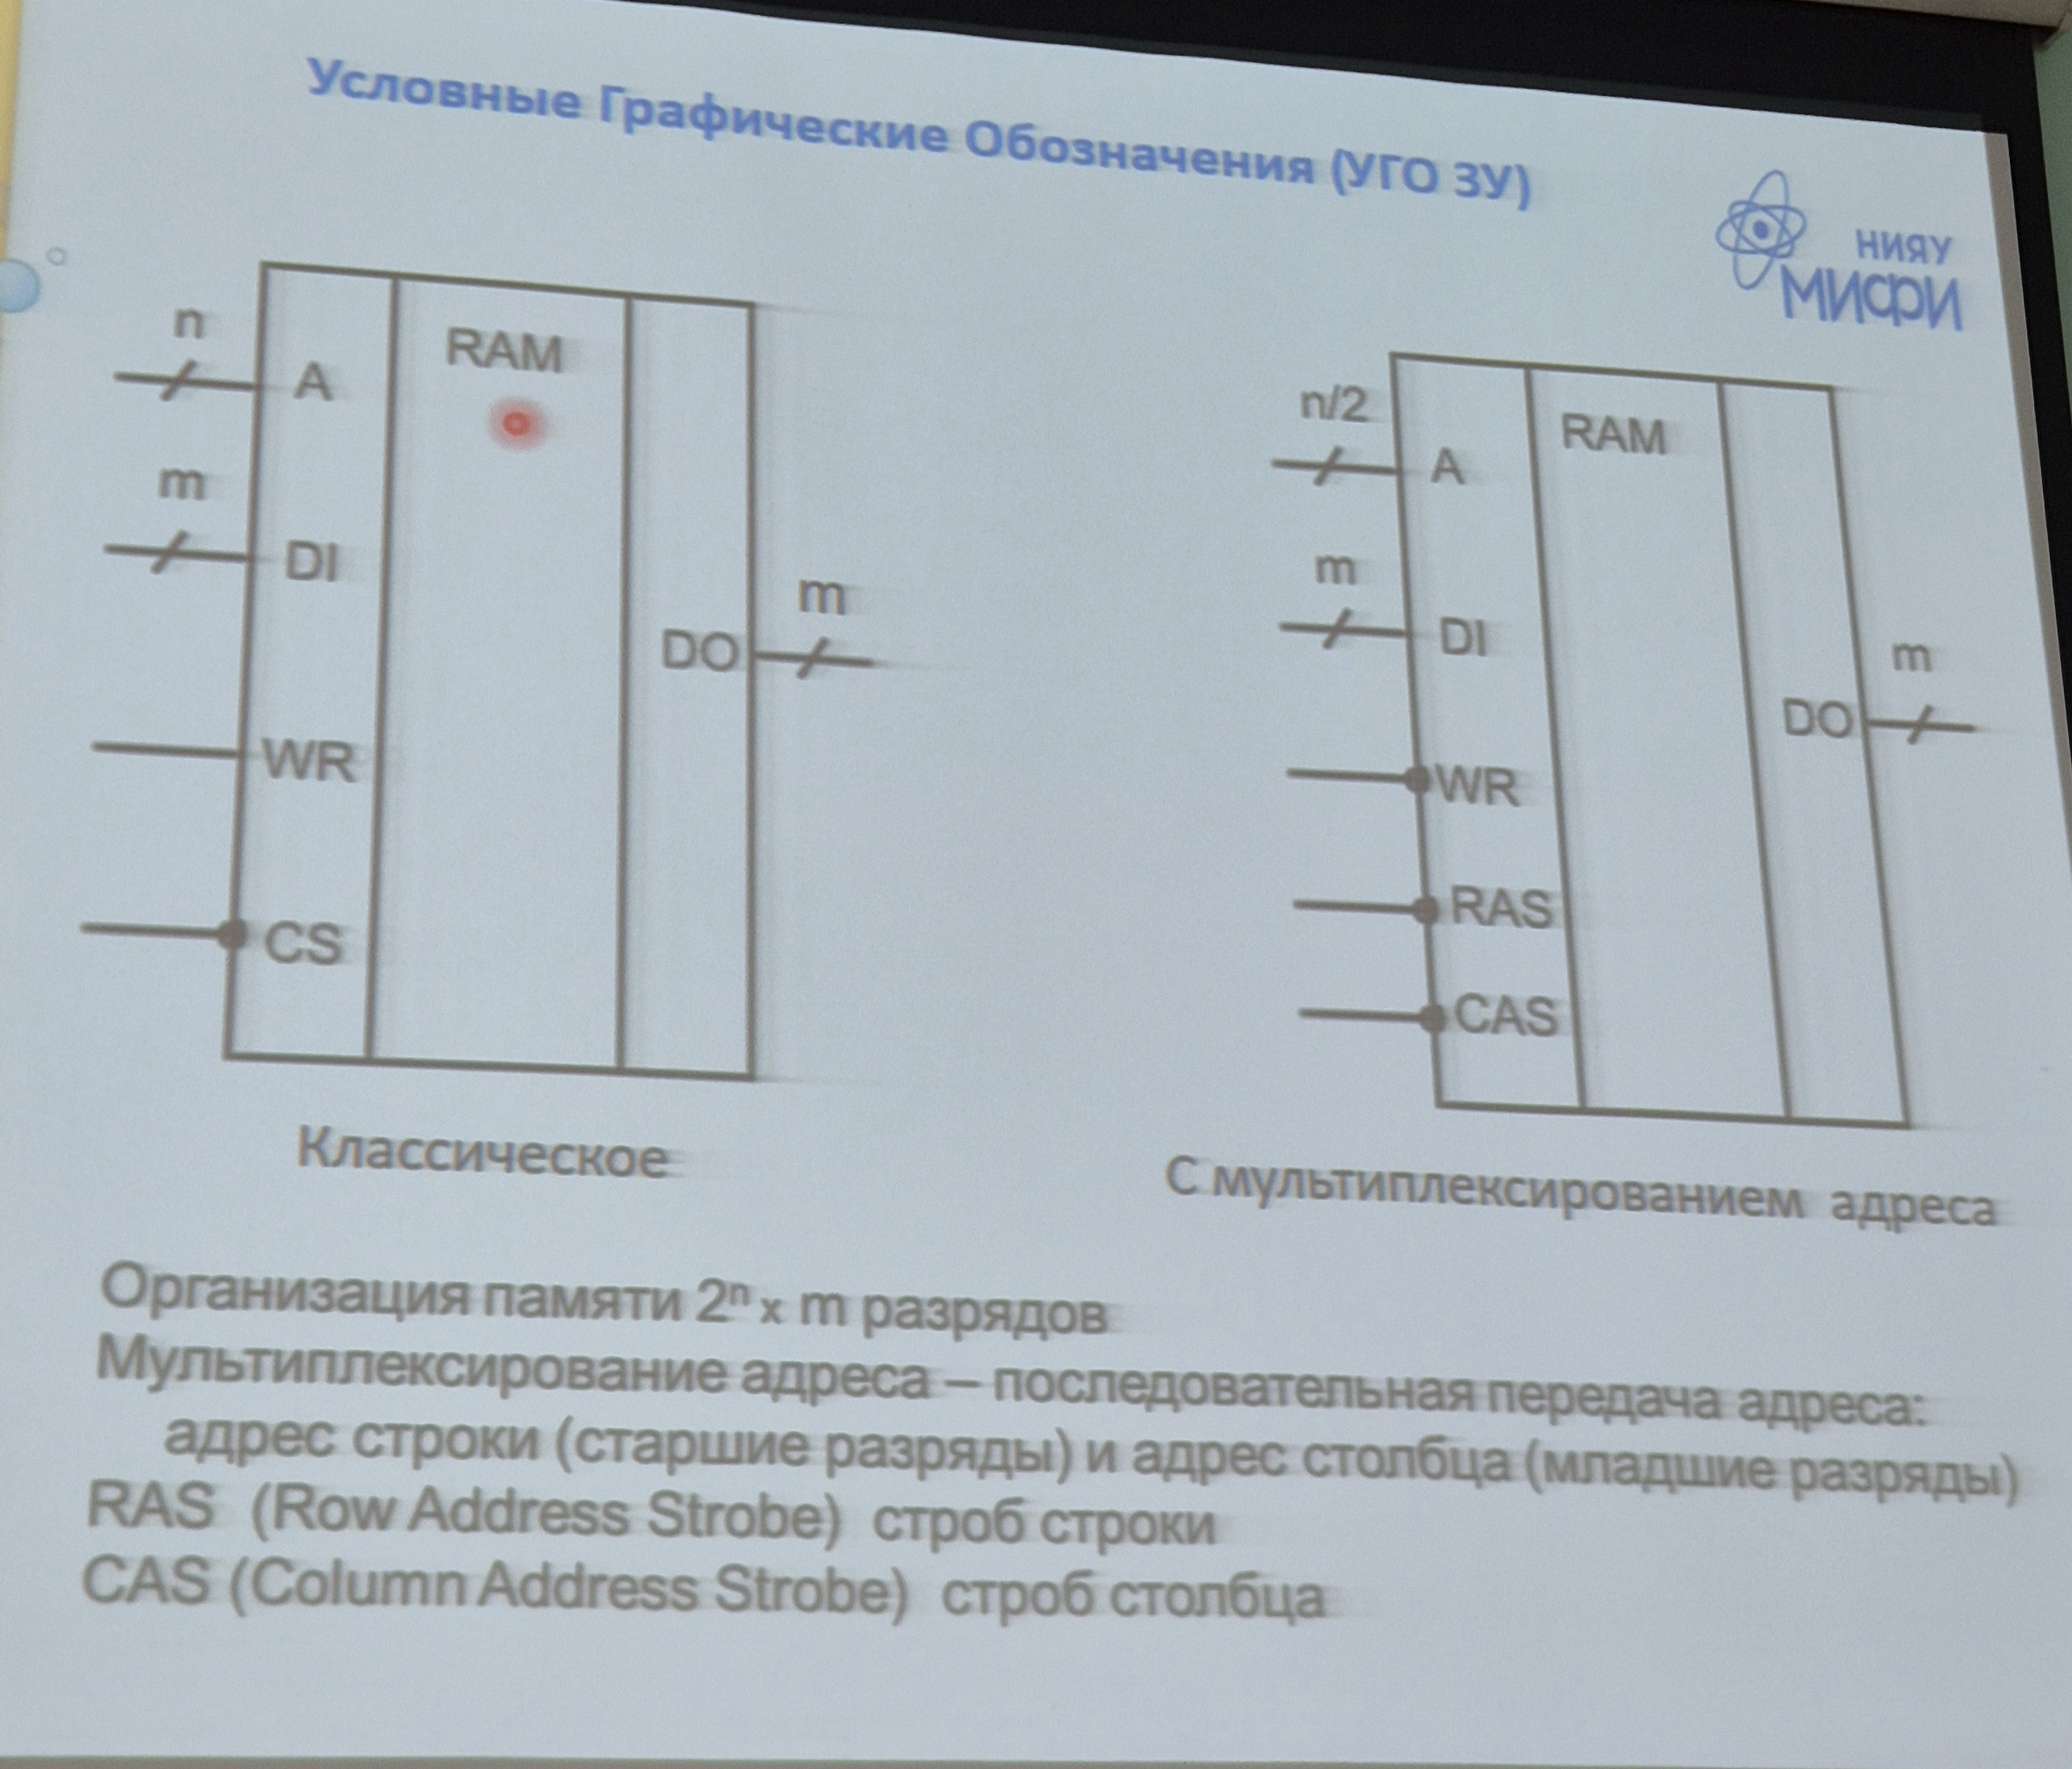
\includegraphics[width=0.7\linewidth]{images/УГО ЗУ.jpg}\\
\end{center}
\textbf{n} - разрядность шины адреса (количество проводов). \\
\textbf{A} - адрес.\\
\textbf{DI} - Data Input. m - размер слова этого запоминающего устройства.\\
\textbf{WR} - Write Read. Какую операцию выполнять\\
\textbf{CS} - Chin Select. Вход разрешения работы этого модуля. Если на схеме выколотая точка, то это означает, что разрешающий сигнал "0".

Организация памяти: $2^n * m$

\section{Семинар 2.}
\subsection{Вопросики (30.10.2025)}
Из скольки частей состоит классическая ЭВМ? - из 3х\\
Какое волшебное слово объясняет, как эти 3 кубика работают? - циклически\\
Предназночение АЛУ? - выполнять АЛ операции.
Что порождает АЛУ? - признак результата и результат. 
что делать - статический сигнал\\
когда делать - импульс\\
Адресуема только вся ячейка, так что любая опреация порисходит сразу со всей ячейкой.\\

\subsection{Продолжаем УГО ЗУ}
DI и DO абсолютно одинаовые\\
Если сигнал на CS не совпадает с разрешающим, то устойство находится в стостоянии хранения. 
\subsection{Организация полупроводникового ЗУ с произвольной выборкой}
\begin{cenetr}
	\includegraphics[width=0.7\linewidth]{images/Полупроводниковое ЗУ.jpg}
\end{cenetr}
\\
Плоская двумерная матрица из запоминающих элементов. 
Бистабильные элементы. \\
Организованно так, чтобы можно было обратиться к люьому элементу. \\
\textbf{Дешифратор} - электронное устройство, преобразующее позиционный двоичный код в код унитарный. \\
\textbf{Унитарный} - двоичный код, содержащий 1 единствуенную единицу. Значение определяется номером разряда, в котором находится единица.\\
Таким образом мы получаем указатель этой единицей на елемент строки или стобца.\\
Регистр хранит 1 число - адрес, которое разделяется на 2 числа пополам, которые считаются номером адреса строки и номером адреса столбца.\\

\subsubsection{Усилители записи считывания}
Правильнее сказать: формировательи.\\
В зависимости от того, из чего сделаны элементы хранений могут быть разные потребности в вольтах и амперах. И суть этих устройств в согласовании внутренних сигналов и внешних стандар	тных логических сигналов. \\

\subsection{Временная диаграмма работы ЗУ RAM.}
\begin{center}
	\includegraphics[width=0.7\linewidth]{images/Временная диаграмма.jpg}
\end{center}

Временная диаграмма - изображение на осях времени электрических сигналов несущих, значения логических переменных. \\

\subsubsection{Запоминающее устройство на фееритовом сердечнике}
\begin{center}
	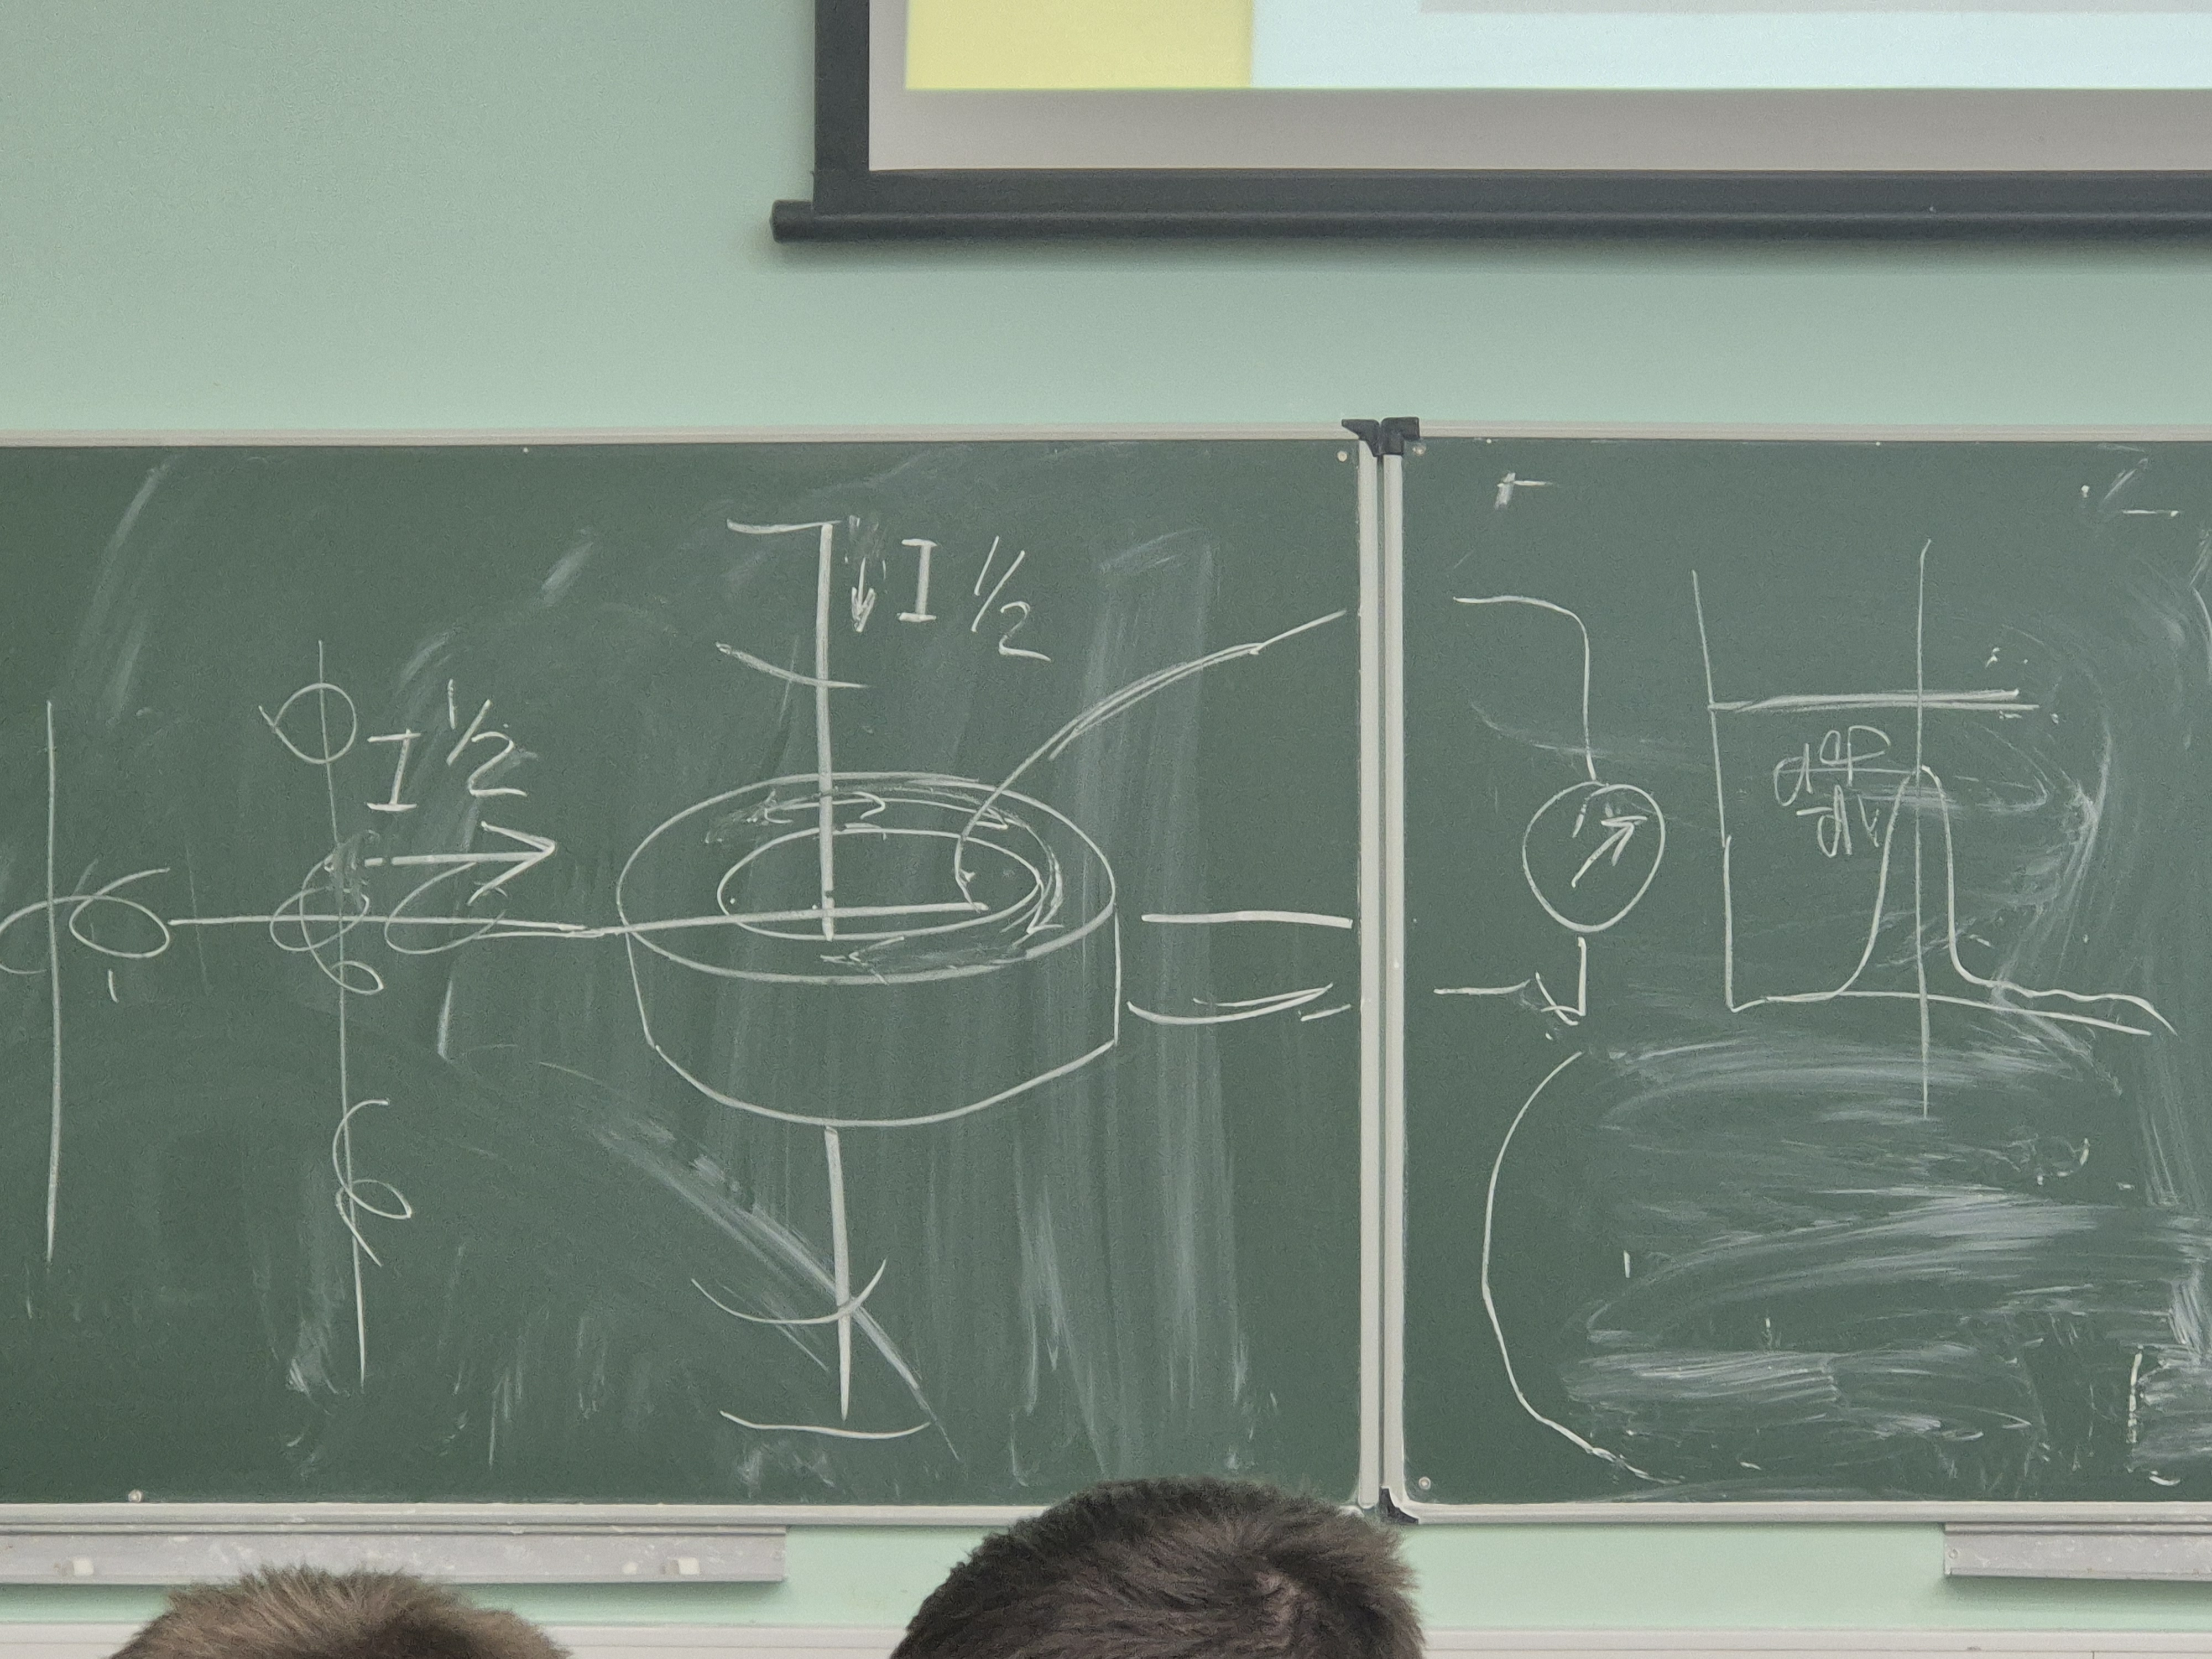
\includegraphics[width=0.7\linewidth]{images/Кольцо.jpg}
\end{center}

Это сплав железа и чем-то ещё так, чтобы получилось хорошо (речь о магнитных свойствах) и испекли пирог в виде кольца. Это кольцо обладает способностью быть намогниченным в двух направлениях
Вокруг тока образуется по правилу буравчика направление намагничивания, а после того

\\
Функции:
\begin{enumerate}
	\item запись ... (всё те же 4)
\end{enumerate}
Запись:\\
Мы пустим половину тока по 1 проволке, а второю половину по второй. (только полный ток перемагнитит). Там где токи пересекаются ячейка переманичеваетя, а другие кольца даже не почешутся. 

Чтение:\\
Пустим 3-ю проволочку (справа кривулька), не пуская по ней ток. 
\begin{enumerate}
	\item Без изменения намагничивания вольтметр ничего не покажет.
	\item При изменении намагничивания возникнет импульс, вольтметр зафиксирует это.
\end{enumerate}
\begin{center}
	\includegraphics[width=0.7\linewidth]{images/Кольцо (слайд).jpg}
\end{center}

Свойства: 
всё равно на радиацию. Разрушить можно только кувалдой. 
\subsection{Ячейка памяти с произвольной выборкой статического типа}
\begin{center}
	\includegraphics[width=0.7\linewidth]{images/SRAM.jpg}
\end{center}

Пара ... выход одного соединён со входом другого. 
Исключает возможность прямого тока от шины питания к земле. Реализован на полевых транзисторах. Хранит только до тех пор, пока есть питание. 
Функции выборки: M5, M6. Они подключены к плечам ячейки и будучи открыты шиной выборки соединяют выбранную ячейку с усилителем, подавая туда 2 сигнала противоположной полярности.\\

Зелёненькое и красненькое на слайдах меняется, поэтому биистабильно :)))\\

Здесь плохо, что ячейка хранит очень мало. 6 транзисторов на 1 бит.\\
Альтернитивный вариант динамическое запоминающее устройство на полевом транзисторе. 

\subsection{Одно-транзисторная ячейка памяти с произвольной выборкой динамического типа.}
\begin{center}
	\includegraphics[width=0.7\linewidth]{images/DRAM.jpg}
\end{center}

Можно использовать конденсатор в качестве элемента хранения.
\begin{center}
	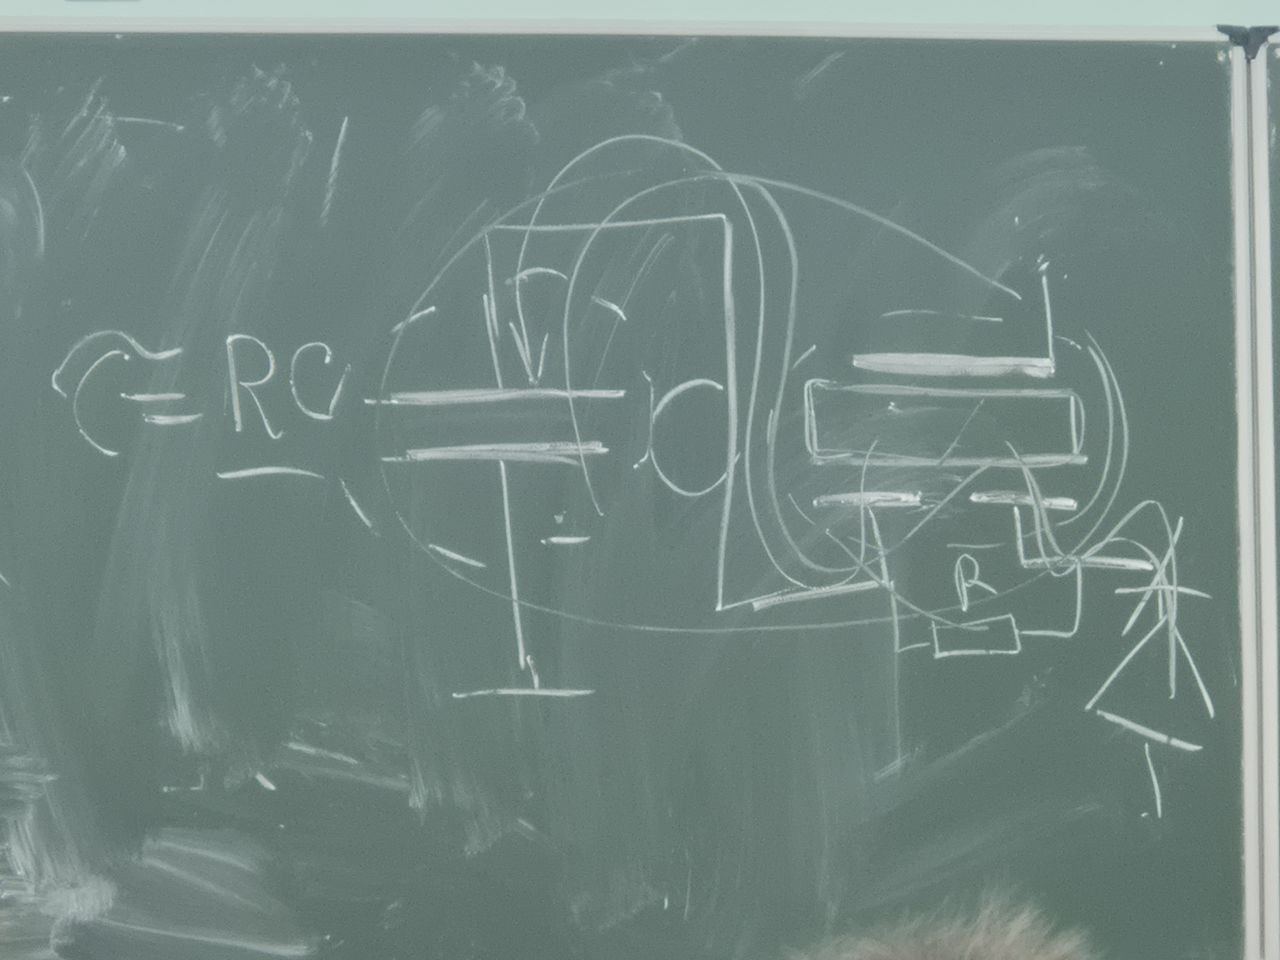
\includegraphics[width=0.7\linewidth]{images/Кондей и полевой транзистор.jpg}
\end{center}
Эквивалентная схемма с открытым транзистором и подключённый к усилителю, а затем закроем транзистор. Если опять открыть, то заряд потечёт в усилитель.\\
Но так как это полуизолятор мы можем повесить дополнительное сопротивление и со временем заряд стечёт и информация будет потеряна. Чтобы этого не произошло нужно считать её, записать и делть это постоянно. \\
Тоесть хранение информации в такой ячейке происходит динамически и требует постоянного чтения и записи (регинирации информаии). 
Почти 90\% всем ЗУ устроены так. \\
Разреженная регинерация - регинерация не всего массива, а только тех, кто нужен. Любое обращение к ячейке вызывает регинирацию.



\end{document}

